The evaluation chapter covers the analysis of the integrated code and the improvements done to the toolkit and the evaluation of CogniCrypt interface to the toolkit. This analysis includes appraisal of the Design Guidelines and interpretation of the results of the metrics of the PUF toolkit for PUF response evaluation. The results of the measurements related to CPU usage and time requirements is presented as
histograms for better assessment of the number of CPU cycles used by the different metrics of the PUF toolkit. For fuzzy extractor techniques the appraisal of the time requirement of the preprcessing  with respect to the parameter $m$ and a PUF response length analysis of the available BCH modes is given.\\

\section{Design Guidelines}
The user interface should be intuitive and easy-to-use which ensures user-satisfaction and effective use to the tool. While extending the toolkit and implementing new metrics, special consideration was given to the user interface design. The existing toolkit followed the standard guidlines as listed in [seb 45] and are summarized below:

\begin{itemize}
	\item \textbf{Simple and natural dialogue:} User must be provided with information related to the task such that the comprehension of the task is natural. The mapping of the user's mental model to the work flow of the toolkit has to be accurate. To satisfy this property the sub-menus are in a top-down structure i.e important options are always in the upper section of each menu. These options are also mandatory eg. the settings like offsets and filenames must be set first before
		progressing to calculation. The sub-menu items after calculation are optional, the toolkit menu follows natural top-down workflow that is inituitive to the user and thus represents a simple and natural dialogue.
	\item \textbf{Speak the user's language:} The intended user group of the toolkit is assumed to be familiar with some technical vocabulary. Translating each and every instruction into laymans langauage distorts the meaning and is not always helpful. So all the dialogues are written as clear instructions with additional examples given to ensure a successful interaction between user and the program.
	\item \textbf{Minimize the user's memory load:} To reduce retyping and user load, all the chosen settings are displayed in each menu. The long inputs like the paths to the different folders can be avoided via explained shortcuts. Common settings like offset needed to be set only once and are applied to all the sub-menus. Additionally brief texts and guidelines to relax the short-term memory of the user are provided that promotes a clear design and visual clarity.
	\item \textbf{Be consistent:} The layout and positioning of the menu items, design concept is consistent throughout and wherever possible exact same words, menu entries and settings options are used for the user to recognize a pattern and prediction of the actions. The control behavior is also consistent, meaning the upper area always shows the important options as mentioned in the text above.
	\item \textbf{Provide Feedback:} The information header in the toolkit informs the user where he/she is in the menu hierarchy. The Feedback and the input area provides with essential information about the result. Not only for errors, but feedback for each performed action and its status is dispayed.
	\item \textbf{Provide clearly marked exits:} The ``exit'' or ``back'' is the lowest menu option in each sub-menu level. This facilitates user yo navigate through the hierarchical structure of the menu or to exit the toolkit.
	\item \textbf{Provide shortcuts:} The selection of each menu entry is implemented as shortcut represented by the corresponding number in front of the option. This helps is fast and spontaneous navigation through the menus.
	\item \textbf{Good error messages:} Whenever user input is incorrect or toolkit is in faulty state, the reason for the error and information to recover from the erroneous state is given in the feedback area. The instructions are simplified and only relevant information to the error with as much detail as possible is presented thereby assisting user for a fast recovery.
	\item \textbf{Prevent errors:} The implementation has a two level check for handling the user inputs to ensure that only legitimate inputs will be processed. Further information related to the input format and representative examples of such sample inputs with brief helper text are displayed to the user for him/her to avoid errors. Exhaustive error checking is performed before calculating the metric to assure that all relevant data and settings are set and valid, so as to prevent
		the program from running into undesired state and crashes.
\end{itemize}

\subsection{CogniCrypt User interface}
The CongniCrypt user interface consists of dialog boxes that ask simple questions to help the Java developers call the functions of the toolkit.
The above mentioned design guidelines were considered for the developement of the UI of CogniCrypt. They not only help to implement a secure Java code for the invocation of the toolkit functions but also assists the developers in getting familiar with the pattern of the toolkit and structure of the PUF responses. For eg. One major question asked by the CogniCrypt to the developer is if he/she wants to evaluate from a single PUF instance or multiple PUF instances (folders), for multiple
folders the CogniCrypts selects Inter-Hamming Distance. Such a question dialog box is represented in the Figure \ref{img:cogni_ui} which shows the simple and inituitive design of the User Interface.\\

\begin{figure}
\centering
\fbox{ 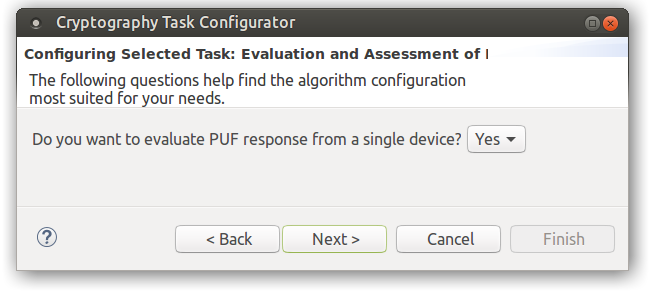
\includegraphics[width=0.97\textwidth]{images/Cogni.png}}
\caption{User interface of the CogniCrypt, represented as a dialog box that asks simple questions for the evaluation of the PUF metrics.}
\label{img:cogni_ui}
\end{figure}

To further enhance the developer experience and improve the UI a survey was taken and the suggestions of the Java developers were integrated in the CogniCrypt. For details of the survey please refer to the research paper [crypto\_icse.pdf]

\section{Interpretation of the results for the extended metrics}
The interpretation for the core metrics that were implemented already in the toolkit are explained in detail in [seb master thesis]. This section presents the interpretation of the extended metrics and also touches upon the hamming weight interpretation since it is a base metric upon which other PUF evaluation metrics are build.
\begin{itemize}
	\item \textbf{Hamming Weight:} This metric was introduced in section \ref{Hamming_Distance_menu} and is used to ensure that a PUF response is not biased towards 0 or 1. For the result to be unbiased, the PUF response evaluation for the Fractional hamming weight metric between two files should be as close to 50\% as possible. Slight deviations are acceptable.
	\item \textbf{Jaccardi Index:} This metric is also sometimes referred to as Jaccard similarity coefficient. As its alternate name suggests the jaccard index measures similarity between two files so the Jaccardi Index should be as close to $1$ or the $Jaccardi Index * 100$ should be as close to 100\% as possible for two files to be similar.
	\item \textbf{Intra-Jaccardi Index:} The general use case for evaluation of the intra-jaccardi Index is when evaluating PUF responses from a single PUF instance with the same particular challenge. Ideally the PUF responses from the same PUF instance and same challenge must be identical, but errors are introduced due to external factors like operating temperature change, voltage fluctuation etc. The PUF response from the same PUF instance are stored in a particular directory and evaluation
		for intra-Jaccardi Index is done for this entire folder. The result for each comparison should be close to $1$ which establishes similarity between files. The fractional Jaccardi Index which is $Jaccardi Index / filesize$ should be close to zero, considering the PUF response sizes are much greater than one byte. Note, slight deviations are tolerable. Another use case for this metric is to gain insight in the uniqueness of the PUF responses from a single PUF instance when
		it is stimulated with different PUF challenges. In such a case the resultant PUF responses should be different from each other depending on the PUF challenge. Note this evaluation only holds ground if the PUF instance offers a challenge space that is greater than one. In this case the Jaccardi Similarity Index should be around $0.5$ (or 50\%) which establishes exclusiveness amongst PUF responses.
	\item \textbf{Inter-Jaccardi Index:} Contrary to the Intra-Jaccardi Index where evaluation of the PUF responses from a single device is done, Inter-Jaccardi Index evaluates PUF responses from multiple devices. As stated above each PUF instance stores the responses in a specific directory, so multiple directories represent multiple PUF instances containing PUF responses which ideally must be similar within the same directory but must be unique and exclusive amongst other directories.
		Therefore the inter Jaccardi Index for the same PUF challenge to different PUF responses from
		seperate PUF instances should be as close to $0.5$ (or 50\%) as possible to ascertain
		uniqueness. Slight deviations from this ideal number are always acceptable.
\end{itemize}

For completeness the table \ref{tab:metrics} summarizes the result interpretation of the metrics with respect to the utilized use case. The table also contains metrics from the original toolkit and are not explained in detail to avoid redudancy. To know more about the metrics in the previous version of the toolkit refer to [seb thesis section evaluation].\\

\begin{table}[!ht]
\centering
\begin{tabular}{@{}lccccc@{}}
\toprule
\multicolumn{1}{l}{\textbf{Metric}}                                                                                             & \multicolumn{1}{c}{\textbf{Instance(s)}} & \multicolumn{1}{c}{\textbf{Challenge(s)}} & \multicolumn{1}{c}{\textbf{Ideal result}}                                         & \multicolumn{1}{c}{\textbf{Deviations}}                                            & \multicolumn{1}{c}{\textbf{Interpretation}}\\
\toprule
\midrule
\multicolumn{1}{l}{\begin{tabular}[c]{@{}l@{}}Hamming \\ weight\end{tabular}}                             & \multicolumn{1}{c}{-}                   & \multicolumn{1}{c}{-}                    & \multicolumn{1}{c}{\begin{tabular}[c]{@{}c@{}}(fractional) \\ 50\%\end{tabular}} & \multicolumn{1}{l}{\begin{tabular}[l]{@{}l@{}}minimal \\ acceptable\end{tabular}} & \multicolumn{1}{l}{\begin{tabular}[l]{@{}l@{}}PUF response \\unbiased\end{tabular}}      \\ \midrule
\multicolumn{1}{l}{\begin{tabular}[c]{@{}l@{}}(Shannon) \\ entropy\end{tabular}}                          & \multicolumn{1}{c}{-}                   & \multicolumn{1}{c}{-}                    & \multicolumn{1}{c}{1}                                                            & \multicolumn{1}{l}{\begin{tabular}[l]{@{}l@{}}minimal \\ acceptable\end{tabular}} & \multicolumn{1}{l}{\begin{tabular}[l]{@{}l@{}}Randomness of \\ PUF response\end{tabular}} \\ \midrule
\multicolumn{1}{l}{\multirow{2}{*}{\begin{tabular}[c]{@{}l@{}}Intra-\\ Hamming \\ distance\end{tabular}}} & \multicolumn{1}{c}{same}                & \multicolumn{1}{c}{same}                 & \multicolumn{1}{c}{\begin{tabular}[c]{@{}c@{}}(fractional) \\ 0\%\end{tabular}}  & \multicolumn{1}{l}{\begin{tabular}[l]{@{}l@{}}minimal \\ acceptable\end{tabular}} & \multicolumn{1}{l}{Reliability}                                                           \\ \cmidrule(l){2-6}
\multicolumn{1}{l}{}                                                                                      & \multicolumn{1}{c}{same}                & \multicolumn{1}{c}{different}            & \multicolumn{1}{c}{\begin{tabular}[c]{@{}c@{}}(fractional) \\ 50\%\end{tabular}} & \multicolumn{1}{l}{\begin{tabular}[l]{@{}l@{}}minimal \\ acceptable\end{tabular}} & \multicolumn{1}{l}{Uniqueness}                                                            \\ \midrule
\multicolumn{1}{l}{\begin{tabular}[c]{@{}l@{}}Inter-\\ Hamming\\ distance\end{tabular}}                   & \multicolumn{1}{c}{different}           & \multicolumn{1}{c}{same}                 & \multicolumn{1}{c}{\begin{tabular}[c]{@{}c@{}}(fractional)\\ 50\%\end{tabular}}  & \multicolumn{1}{l}{\begin{tabular}[l]{@{}l@{}}minimal\\ acceptable\end{tabular}}  & \multicolumn{1}{l}{Uniqueness}                                                            \\ \midrule
\multicolumn{1}{l}{\multirow{3}{*}{\begin{tabular}[c]{@{}l@{}}Min-\\ entropy\end{tabular}}}               & \multicolumn{1}{c}{same}                & \multicolumn{1}{c}{same}                 & \multicolumn{1}{c}{0}                                                            & \multicolumn{1}{l}{\begin{tabular}[l]{@{}l@{}}minimal \\ acceptable\end{tabular}} & \multicolumn{1}{l}{\begin{tabular}[l]{@{}l@{}}Robustness /\\Reliability\end{tabular}}    \\ \cmidrule(l){2-6}
\multicolumn{1}{l}{}                                                                                      & \multicolumn{1}{c}{different}           & \multicolumn{1}{c}{same}                 & \multicolumn{1}{c}{\begin{tabular}[c]{@{}c@{}}(fractional)\\ high\end{tabular}}  & \multicolumn{1}{l}{\begin{tabular}[l]{@{}l@{}}minimal\\ acceptable\end{tabular}}  & \multicolumn{1}{l}{Uniqueness}                                                            \\ \cmidrule(l){2-6}
\multicolumn{1}{l}{}                                                                                      & \multicolumn{1}{c}{same}                & \multicolumn{1}{c}{same}                 & \multicolumn{1}{c}{\begin{tabular}[c]{@{}c@{}}(fractional)\\ high\end{tabular}}  & \multicolumn{1}{l}{\begin{tabular}[l]{@{}l@{}}minimal\\ acceptable\end{tabular}}  & \multicolumn{1}{c}{\begin{tabular}[l]{@{}l@{}}Noise extraction\\ possible\end{tabular}}   \\
\midrule

\multicolumn{1}{l}{\begin{tabular}[c]{@{}l@{}}Jaccardi \\ Index\end{tabular}}                             & \multicolumn{1}{c}{-}                   & \multicolumn{1}{c}{-}                    & \multicolumn{1}{c}{100\%} & \multicolumn{1}{l}{\begin{tabular}[l]{@{}l@{}}minimal \\ acceptable\end{tabular}} & \multicolumn{1}{l}{\begin{tabular}[l]{@{}l@{}}PUF response \\similarity\end{tabular}}      \\ \midrule
\multicolumn{1}{l}{\multirow{2}{*}{\begin{tabular}[c]{@{}l@{}}Intra-\\ Jaccardi \\ Index\end{tabular}}} & \multicolumn{1}{c}{same}                & \multicolumn{1}{c}{same}                 & \multicolumn{1}{c}{\begin{tabular}[c]{@{}c@{}}(fractional) \\ 0\%\end{tabular}}  & \multicolumn{1}{l}{\begin{tabular}[l]{@{}l@{}}minimal \\ acceptable\end{tabular}} & \multicolumn{1}{l}{Reliability}                                                           \\ \cmidrule(l){2-6}
\multicolumn{1}{l}{}                                                                                      & \multicolumn{1}{c}{same}                & \multicolumn{1}{c}{different}            & \multicolumn{1}{c}{50\%} & \multicolumn{1}{l}{\begin{tabular}[l]{@{}l@{}}minimal \\ acceptable\end{tabular}} & \multicolumn{1}{l}{Uniqueness}                                                            \\ \midrule
\multicolumn{1}{l}{\begin{tabular}[c]{@{}l@{}}Inter-\\ Jaccardi\\ Index\end{tabular}}                   & \multicolumn{1}{c}{different}           & \multicolumn{1}{c}{same}                 & \multicolumn{1}{c}{50\%}  & \multicolumn{1}{l}{\begin{tabular}[l]{@{}l@{}}minimal\\ acceptable\end{tabular}}  & \multicolumn{1}{l}{Uniqueness}                                                            \\ \midrule

\addlinespace
\bottomrule
\end{tabular}
\caption{Extended version of the table showing Interpretation of the results regarding the metrics in dependency to the utilized use case.}
\label{tab:metrics}
\end{table}

\textbf{Time requirements:} To test the new metrics of the toolkit an analysis of the time taken by the calculation APIs for the PUF response evaluation of multiple instances was performed. The time taken by the user to input the settings was skipped, the measurement of the time was done using the standard ``clock()'' API of the GNU C library which is used to determine the process time (refer to manpage of clock for more detail). For testing, the SRAM PUF responses from Texas Instrument (TI) Stellaris LM4F120XL LaunchPad Evaluation Kits with a
size of 32 Kilobytes and an offset of 400 bytes from beginning were used. The analysis was performed on an Intel i3 quad core CPU with 2.00 GHz and 3 GB RAM. The results of the time requirements for Intra Jaccardi Index and Inter Jaccardi Index are visualized in Figures \ref{img:time_intra} and \ref{img:time_inter} respectively. The time taken analysis for the Jaccardi Index is not represented since it is constant around $0.7$ milliseconds.

\begin{figure}
\centering
%\fbox{ \includegraphics[width=0.97\textwidth]{images/time2a.png}}
\caption{Time requirement measurements of the \emph{Intra-Jaccardi Index}.}
\label{img:time_intra}
\end{figure}

\begin{figure}
\centering
%\fbox{ \includegraphics[width=0.97\textwidth]{images/time2a.png}}
\caption{Time requirement measurements of the \emph{Inter-Jaccardi Index}.}
\label{img:time_inter}
\end{figure}

\subsection{Evaluation of the Fuzzy extractor}
To evaluate the fuzzy extractor we compare both the coding techniques, Golay Code and BCH code used in the fuzzy implementation. Both of which are assisted with linear repetition algorithm and majority voting procedure. The error correction capability $t$ of golay code is limited to maximum of three bit errors for a message length of \emph{12 bits}. Both the codes are linear codes so they take the same parameters (n, k, d), where $n$ is the length (in bits) of the encoded codeword, $k$ is the
length (message length) of the input secret/message that is fed to the encoder and $d$ is the minimal hamming distance from which the error correcting capablity is derived using the formula $t = \lfloor(d-1)/2\rfloor$. The golay code uses a lookup table to encode the \emph{12 bits} of message to \emph{23 bits} of codeword, incase there are more than three bits of errors introduced while processing PUF instance for response (due to external noise and environmental factors) then the decoding lookup
table for golay code is not capable to correct errors which leads to an undesired state. To avoid this behavior, the user is presented with an error message that it is out of Golay code's scope to correct so many errors and to use BCH coding instead.

The BCH coding implementation on the contrary corrects as many bit errors as possible in each codeword. If errors exceed the correction capability $t$ of the BCH code then only $t$ errors are corrected and remaining errors are ignored. This avoids the undesired behavior unlike the golay code and the information about the detected but not corrected errors is displayed to the user which enhances the robustness of the fuzzy extractor. In addition, the paramters of the BCH code are
highly configurable and can be adjusted to the noise level that introduces the errors. The pre evaluation of the PUF responses from the PUF instances can be utilized to predict the error correction capability and the parameters of the BCH code can be adjusted accordingly to ensure a reliable working procedure. The table \ref{tab:BCHmodes} list the possible paramters that are valid of the BCH(n, k, d) code.\\

\begin{table}[!ht]
\small
\begin{center}
\begin{tabular}{rrrr|rrrr|rrrr|rrrr}
\toprule
\multicolumn{16}{c}{\textbf{Common BCH codes of order less than $2^{10}$}}\\
\midrule
\hline
n & k & d & t & n & k & d & t & n & k & d & t & n & k & d & t \\
\hline
7&4&3&1&127&8&63&31&511&484&7&3&511&166&95&47\\
15&11&3&1&255&247&3&1&&475&9&4&&157&103&51\\
&7&5&2&&239&5&2&&466&11&5&&148&107&53\\
&5&7&3&&231&7&3&&457&13&6&&139&109&54\\
31&26&3&1&&223&9&4&&448&15&7&&130&111&55\\
&21&5&2&&215&11&5&&439&17&8&&121&117&58\\
&16&7&3&&207&13&6&&430&19&9&&112&119&59\\
&11&11&5&&199&15&7&&421&21&10&&103&123&61\\
&6&15&7&&191&17&8&&412&23&11&&94&125&62\\
63&57&3&1&&187&19&9&&403&25&12&&85&127&63\\
&51&5&2&&179&21&10&&394&27&13&&76&171&85\\
&45&7&3&&171&23&11&&385&29&14&&67&175&87\\
&39&9&4&&163&25&12&&376&31&15&&58&183&91\\
&36&11&5&&155&27&13&&367&33&16&&49&187&93\\
&30&13&6&&147&29&14&&358&37&18&&40&191&95\\
&24&15&7&&139&31&15&&349&39&19&&31&219&109\\
&18&21&10&&131&37&18&&340&41&20&&28&223&111\\
&16&23&11&&123&39&19&&331&43&21&&19&239&119\\
&10&27&13&&115&43&21&&322&45&22&&10&255&127\\
&7&31&15&&107&45&22&&313&47&23&1023&1013&3&1\\
127&120&3&1&&99&47&23&&304&51&25&&1003&5&2\\
&113&5&2&&91&51&25&&295&53&26&&993&7&3\\
&106&7&3&&87&53&26&&286&55&27&&983&9&4\\
&99&9&4&&79&55&27&&277&57&28&&973&11&5\\
&92&11&5&&71&59&29&&268&59&29&&963&13&6\\
&85&13&6&&63&61&30&&259&61&30&&953&15&7\\
&78&15&7&&55&63&31&&250&63&31&&943&17&8\\
&71&19&9&&47&85&42&&241&73&36&&933&19&9\\
&64&21&10&&45&87&43&&238&75&37&&923&21&10\\
&57&23&11&&37&91&45&&229&77&38&&913&23&11\\
&50&27&13&&29&95&47&&220&79&39&&903&25&12\\
&43&29&14&&21&111&55&&211&83&41&&893&27&13\\
&36&31&15&&13&119&59&&202&85&42&&883&29&14\\
&29&43&21&&9&127&63&&193&87&43&&873&31&15\\
&22&47&23&511&502&3&1&&184&91&45&&863&33&16\\
&15&55&27&&493&5&2&&175&93&46&&858&35&17\\
\hline
\addlinespace
\bottomrule
\end{tabular}
\end{center}
\caption{BCH codes generated by primitive elements of order less than $2^{10}$ and the corresponding parameters \emph{n}, \emph{k} \emph{d} and \emph{t}.}
\label{tab:BCHmodes}
\end{table}

\subsection{Pre-evaluation Relevance}
\emph{\textbf{PUF response length analysis:}} To select the optimal BCH mode parameters it is important to ascertain the length of the PUF response which also forms a part of pre-evaluation phase. The PUF response length is based on the size of the input secret and parameters $k$ and $d$ of the BCH code alongwith the Linear repetition factor selected for encoding. The PUF response length that satisfies the BCH code selection paramters can be verified using the Equation
		\ref{PUF_length}.
\begin{itemize}
	\item The size of the input secret is $N$ bits, the BCH parameters corresponds to the chosen BCH(n, k, d) mode and the linear repetition factor is denoted with LR (7 or 15). The required length of the PUF reponse is represented with the symbol \emph{RequiredPUFLength}[seb thesis].\\
		\begin{equation}
			RequiredPUFLength \geq \Bigg\lceil\Bigg(\dfrac{\Bigg(\Bigg\lceil\dfrac{N}{k}\Bigg\rceil
		* n\Bigg)}{8}\Bigg)\Bigg\rceil * LR
		\label{PUF_length}
		\end{equation}
\end{itemize}

The pre-evaluation is inevitable for an effective and efficient development of PUF-based security approaches and it should be included in the developement cycle of the PUF-based security algorithms. The pre-evaluation of the TI Stellaris LM4F120XL Launchpad Kit showed that the complete SRAM from this hardware cannot be considered as a PUF, because of the boot process which effects the randomness of the first  $400$ bytes and renders these bytes not to be considered a part of the PUF response.
Without pre-evaluation such exceptional behavior cannot be discovered which could result in an insecure implementation of the PUF-based security approaches. For determining the required error correction capability of the BCH code, the pre-evaluation of the PUF instance is critical for the selection of the optimal parameters. These two scenarios illustrate that the pre-evaluation must be considered as a decisive factor in the developement of the PUF-based security appraches.


\section{Time requirement analysis}

The BCH code is highly configurable that means the parameters m, n, t can be constructed in various possible ways. For time requirement analysis the preprocessing time for the generation of a BCH mode was taken into account. Depending on the selected parameters, specifically $m$, the preprocessing can create some timing overhead. Since this process is inevitable for both encoder and decoder, the timing overhead is considered with respect to the selection of the parameters, especially since
the adaptation of the fuzzy extractor is intended for hardware machine with limited resources. For testing, all possible m (in range [4,14]), the corresponding maximum n ( $2^{n-1} - 1 < n <= 2^{n} - 1$) and the highest possible error correction capability t were chosen. The time requirement analysis was performed on an Intel i3 quad core CPU with 2.0 GHz and 3 GB RAM. The results of the time measurements for the BCH mode pre-processing are visualized in Figure \ref{img:bch_time}.

The golay code is a static (23, 12, 7) code where the user is not required to input any parameters. The pre-processing time of the golay code remains constant and is not an timing overhead, so it can be ignored. The time required for encoding and decoding steps depends on the size of the file that is to be encoded/decoded. For the analysis we used a PUF response from (TI) Stellaris LM4F120XL LaunchPad Evaluation Kits and the size was varied with the help of offsets, the original size of
the PUF response was 32 Kilobytes. The Figure \ref{img:golay_enc_time} and \ref{img:golay_dec_time} illustrates the encoding and decoding analysis of golay code as a histogram respectively.\\

\begin{figure}
\centering
%\fbox{ 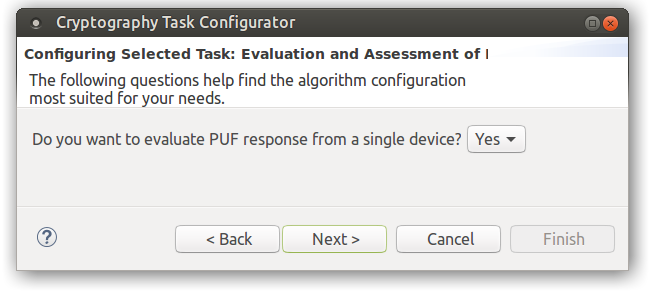
\includegraphics[width=0.97\textwidth]{images/Cogni.png}}
\caption{Time requirement measurements for the BCH mode pre-processing in relation to parameter m.}
\label{img:bch_time}
\end{figure}


\begin{figure}
\centering
%\fbox{ 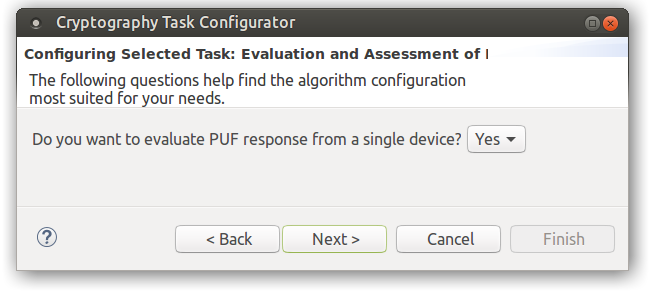
\includegraphics[width=0.97\textwidth]{images/Cogni.png}}
\caption{Time requirement measurements for the Golay encoding for varying filesizes}
\label{img:golay_enc_time}
\end{figure}

\begin{figure}
\centering
%\fbox{ 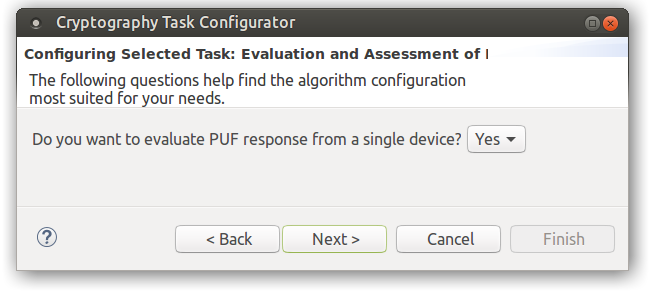
\includegraphics[width=0.97\textwidth]{images/Cogni.png}}
\caption{Time requirement measurements for the Golay decoding for varying filesizes}
\label{img:golay_dec_time}
\end{figure}
